\section{Further Optimization \\and Improvements}
\label{sec:ceph-tuning}

\subsection{Improving RADOS Performance}

\begin{figure}[h]
\centering
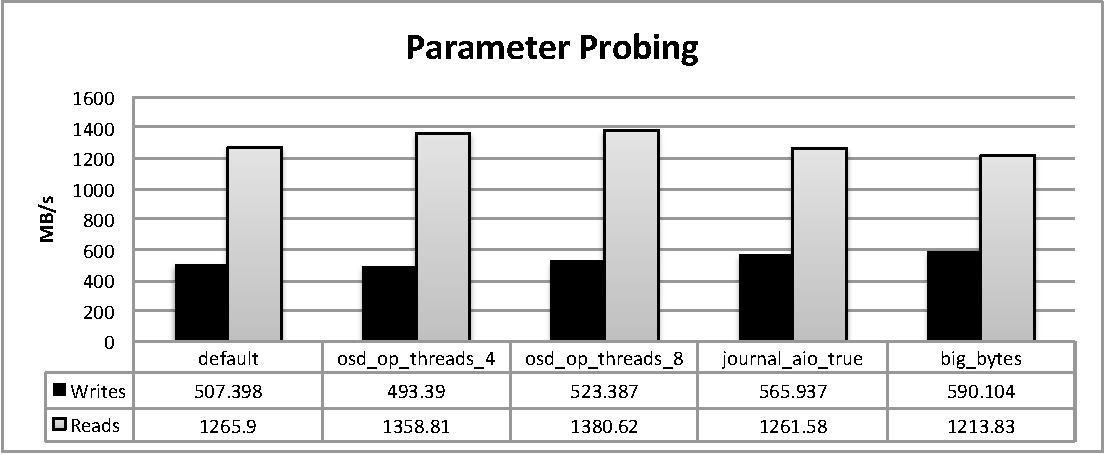
\includegraphics[width=3.5in]{para2}
%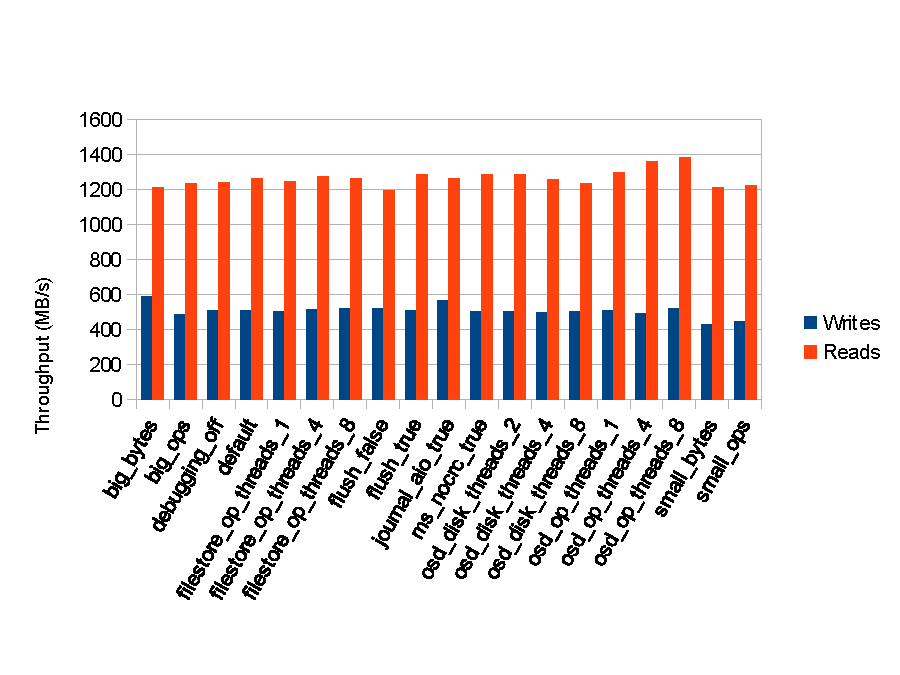
\includegraphics[width=3.5in]{parametric}
\caption{Evaluating parameter impact through sweeping test}
\label{fig:parametric}
\end{figure}

After the initial test results, we tried various combinations of tweaks
including: changing the number of filestore op threads, putting all of the
journals on the same disks as the data, doubling the OSD count, and upgrading
Ceph to a development version which reduces the seek overhead caused by
\texttt{pginfo} and \texttt{pglog} updates on XFS (these enhancements are now
included as of the Ceph Cuttlefish release, v0.61).  

%The two biggest
%improvements resulted from disabling CRC32c checksums and increasing the OSD
%count on the server.  With these changes, we are seeing better results.

We swept over Ceph configuration parameters to examine how different tuning
options affect performance on the DDN platform. The result of this parameter
probing is illustrated in Figure~\ref{fig:parametric}. Please refer to
Appendix E of \cite{ceph:techreport} for explanations of these probed
parameters. In this figure, the default is where we started with. Reads
benefit from increasing the \verb!osd_op_threads! (4 and 8), with 7.3\% and
9\% improvement respectively. For writes, the substantial boost comes with
\verb!journal_aio! true and \verb!big_bytes!, with 11.5\% and 16.3\%
improvement respectively. Other probed parameters (not shown on this figure)
doesn't bear tangible impacts.


%As a result of this testing, we improved performance slightly by
%increasing the size of various Ceph buffers and queues, enabling AIO journals,
%and increasing the number of OSD op threads.

\begin{comment}

\subsubsection{Disable Cache Mirroring on Controllers}

During a second round of test performed by Inktank, we noticed a dramatic drop
on RADOS performance: even though write throughput on individual server met the
expectation, it did not scale across servers.

We spent a significant amount of time
investigating this phenomenon. Ultimately, we were able to replicate this finding
when running concurrent disk throughput tests directly on the servers without
Ceph involved. The second RAID processor on each DDN controller would max out when
three or more LUNs were written concurrently. It turns out the root of the problem
was a regression on DDN firmware update -- in particular, the cache
mirroring was not behaving as it should.\footnote{DDN recently released a new
firmware version and we were told the issue has been fixed. Unfortunately, we didn't get
a chance to verify it during our test cycle.}

%% SCOTT - is running with cache mirroring off and option for a production system or not?
%% What are the consequences? Did DDN eventually provide a fix? If yes, were we able to test
%% with it or not?

%% FEIYI: add footnote to clarify the issue.

\begin{figure}[htb]
\centering
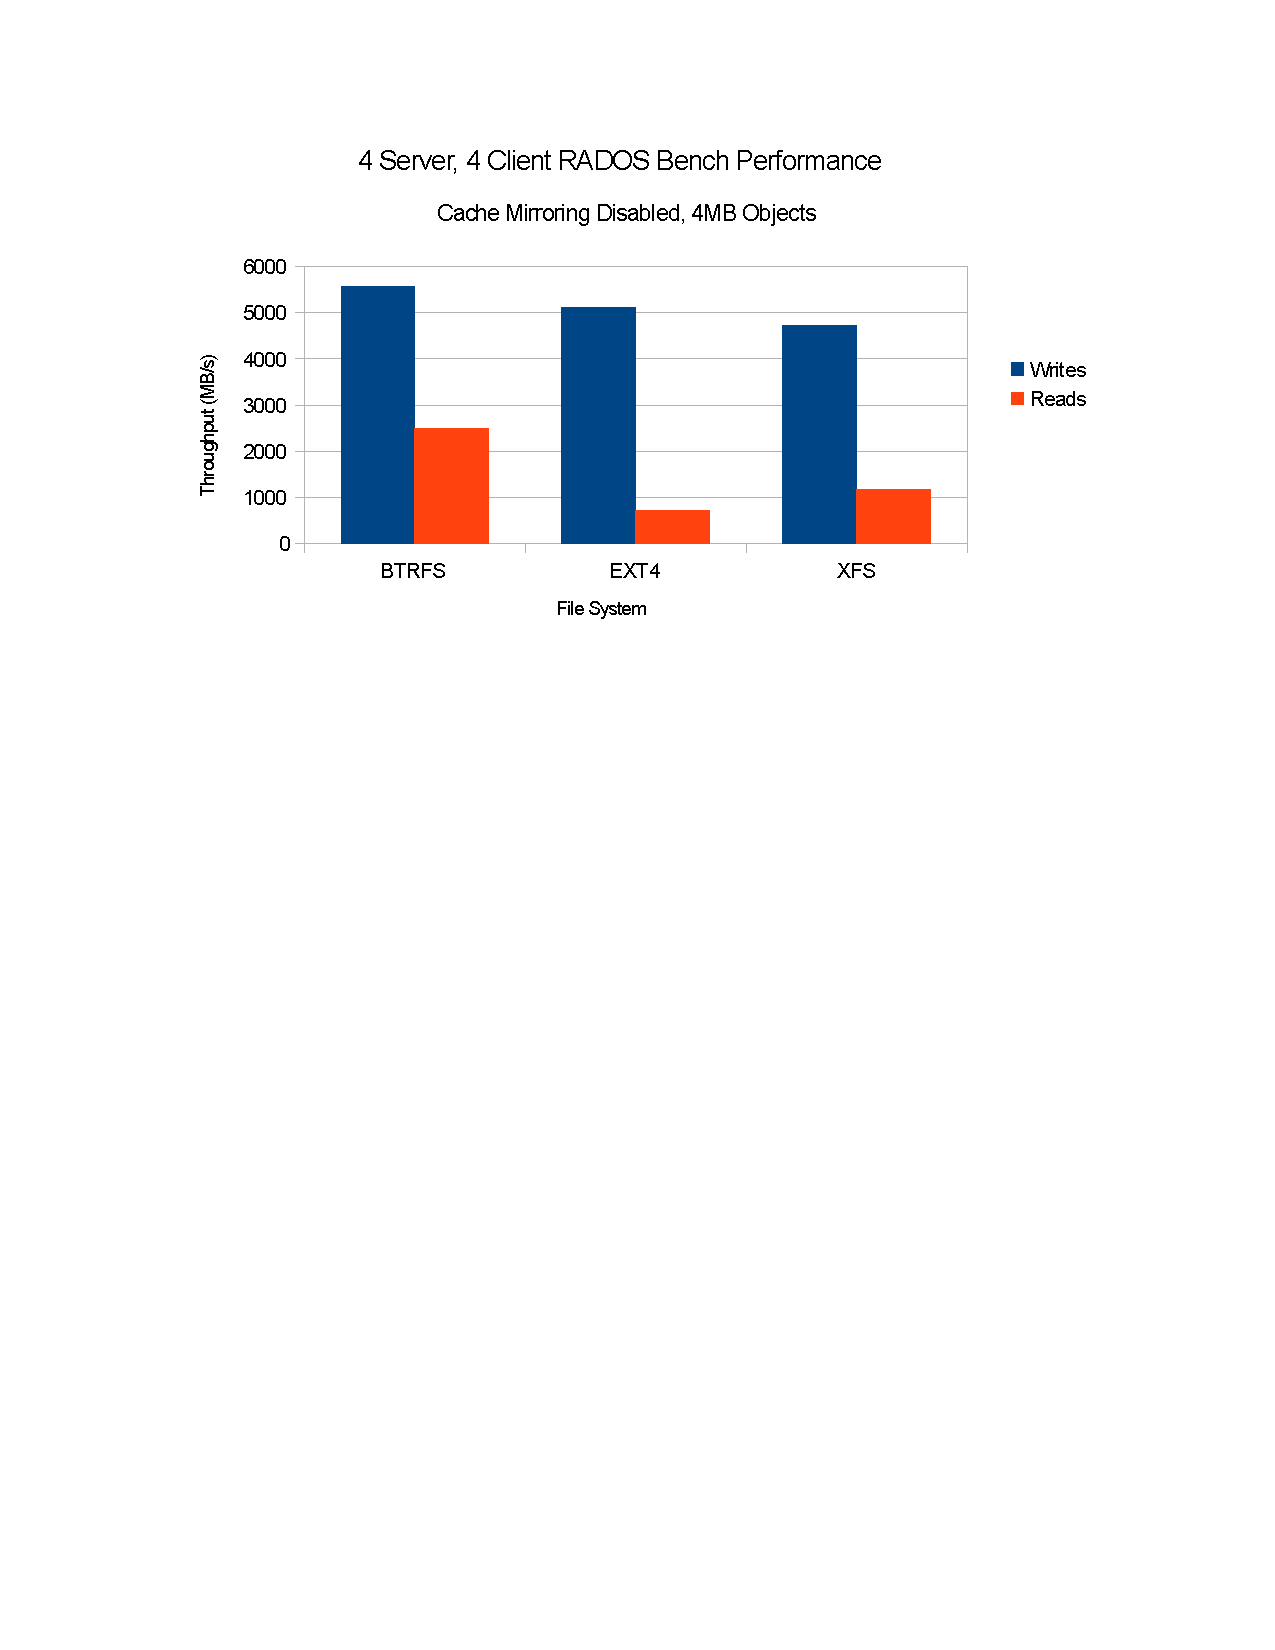
\includegraphics[width=3.5in]{rados-after-ddn}
\caption{Evaluating RADOS bench after disabling cache mirroring}
\label{fig:rados-ddn-mirror-disabled}
\end{figure}


With cache mirroring disabled, write performance when using all four servers
improved dramatically, as illustrated in
Figure~\ref{fig:rados-ddn-mirror-disabled}. With BTRFS, for example, we hit over
5.5 GB/s from the clients.  When accounting for journal writes, that is over
11 GB/s to the disks and very close to what the DDN chassis is capable of doing. 
Unfortunately, read performance did not scale as well.


\subsubsection{Repeating RADOS Scaling Test}

We now repeated the previous RADOS scaling tests with these improvements in place.
The first test was done on a single node with RADOS Bench to see how close the
underlying object store could get to the node hardware limitations as the number
of OSDs/LUNs used on the node increased. All the tests performed were against
XFS-formatted storage.

%% SCOTT - the title in the figure needs to change IO to I/O

%% SCOTT - how do writes inc. journals exceed the client network max? Dual ports
%% on the single server?

\begin{figure}[htb]
\centering
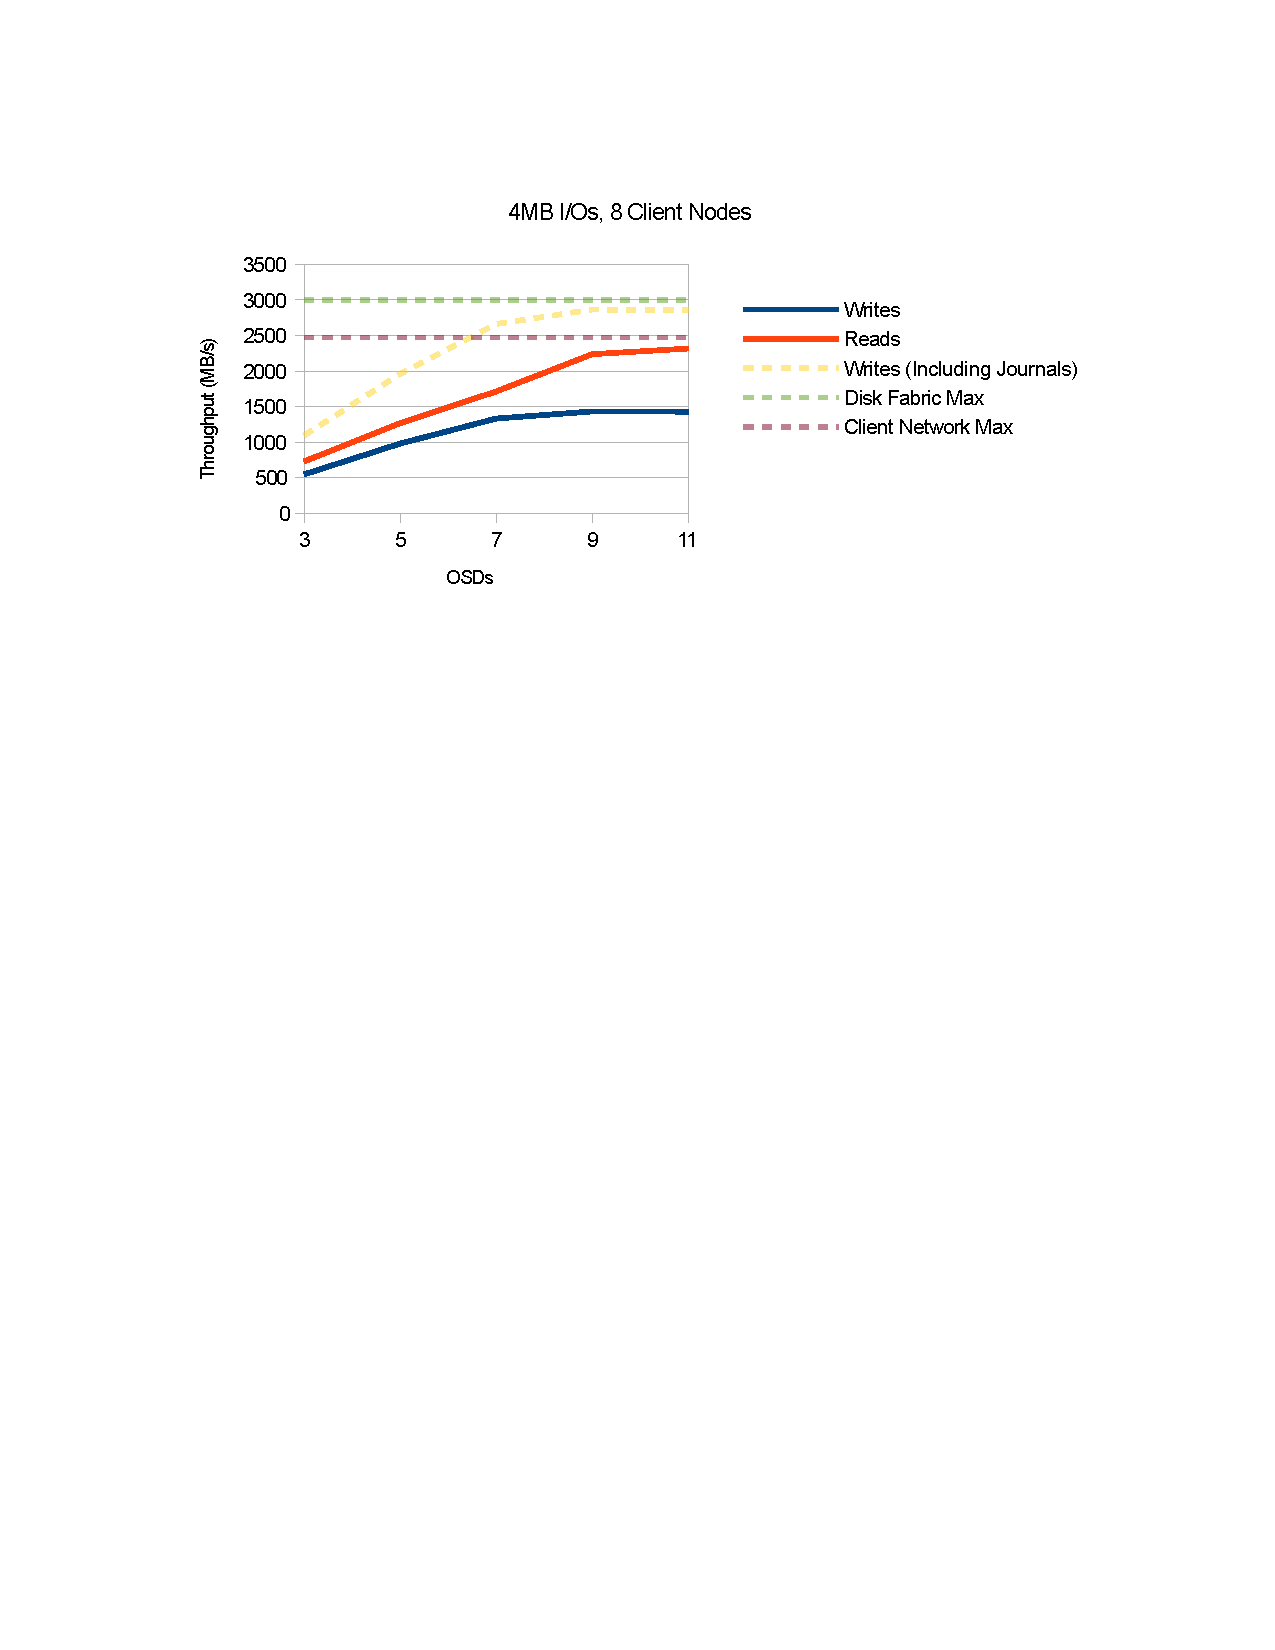
\includegraphics[width=3.5in]{rados-064-osd}
\caption{RADOS Bench Scaling on number of OSD, Ceph 0.64, 4 MB I/O, 8 Client Nodes}
\label{fig:rados-064-osd}
\end{figure}

In the single server case as shown in Figure~\ref{fig:rados-064-osd}, ``Writes
(including Journals)'' refers to how much data is actually being written out
the DDN SFA10K (observed directly from the controllers), and blue line is how
much data the clients are writing.  We observe that performance observed by the
DDN controllers gets very close to the hardware limits at roughly 9 OSDs per
server and then mostly levels out.

We also repeated tests looking at RADOS Bench performance as the number of OSD
server nodes increases from one to four. The results are summarized in
Figure~\ref{fig:rados-064-oss}. As the number of nodes increases, performance
scales nearly linearly for both reads and writes.

%% SCOTT - why does the client network max scale in figure 12 but not figure 11?
%% Do they no measure the same thing (i.e. a single server)? If not, the text
%% needs to make it more clear.

\begin{figure}[htb]
\centering
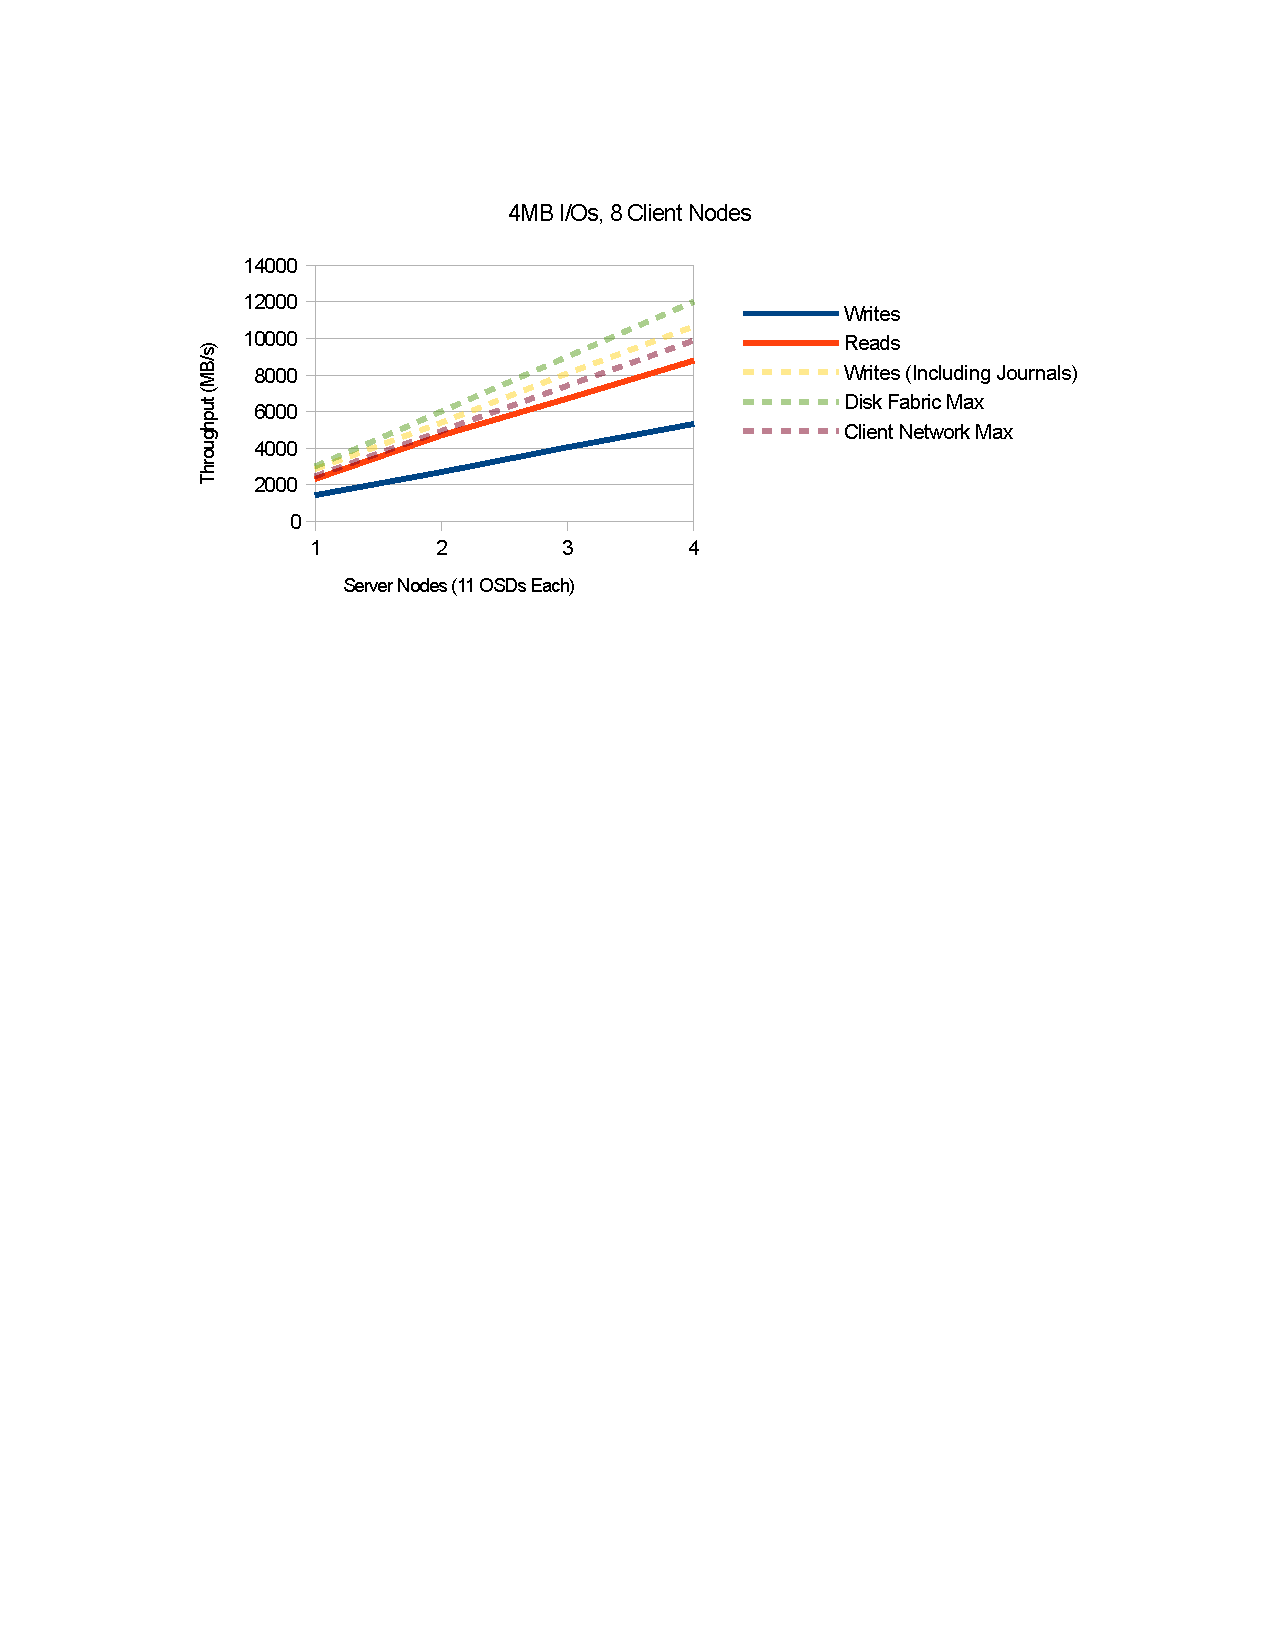
\includegraphics[width=3.5in]{rados-064-oss}
\caption{RADOS Bench Scaling on number of servers, Ceph 0.64, 4 MB I/O, 8 client
nodes}
\label{fig:rados-064-oss}
\end{figure}

\end{comment}



\subsection{Improving Ceph File System Performance}
\label{sec:ceph-tuning-fs}

The initial stability issues mentioned in Section~\ref{sec:ior-initial} are
fixed by migrating from Ceph version 0.48/0.55 to 0.64, the latest stable
version at the time of writing this report.  Upgrading to the latest stable
Ceph release allowed us to run a full IOR parameter sweep for the first time
since we started evaluating the performance and scalability of the Ceph file
system.  This is another sign of how much Ceph development is currently in
flux.

%%%%%%%%%%%%%%%%%%%%%%%%%%%%%%%%%%% removed for space

\begin{comment}

Another fix introduced by Ceph version 0.64 was in pool creation.  The default
data pool used by previous Ceph version were set to 2x replication by mistake.
This potentially halved the write performance. With version 0.64 we explicitly
set the replication level to 1, which is the preferred value for a HPC
environment like ours running on high-end and reliable storage backend hardware
(e.g. DDN SFA10K).

\end{comment}


Even with these changes in place, less-than-ideal write performance and very
poor read performances were observed during our tests.  We also observed that
by increasing the number of IOR processes per client node, the read
performance degraded even further indicating some kind of contention either on
the clients or on the OSD servers.


\subsubsection{Disabling Client CRC32}

At this point, we were able to both make more client nodes available for Ceph
file system-level testing and also install a profiling tool called \verb!perf!
that is extremely useful for profiling both kernel and user space codes.
Profiling with \verb!perf! showed high CPU utilization on test clients due to
CRC32c processing in the Ceph kernel client.  

%%%%%%%%%%%%%%%%%%%%%%%%%%%%%%%%%% removed

%CRC32 checksums can be disabled
%by changing the CephFS mount options:

%\begin{Verbatim}[fontsize=\small]
%mount -t ceph 10.37.248.43:6789:/ 
%    /mnt/ceph -o name=admin,nocrc
%\end{Verbatim}


With client CRC32 disabled, we repeated the IOR tests. New results are shown in
in Figure~\ref{fig:ior-no-client-crc32}. 

\begin{figure}[htb]
\centering
%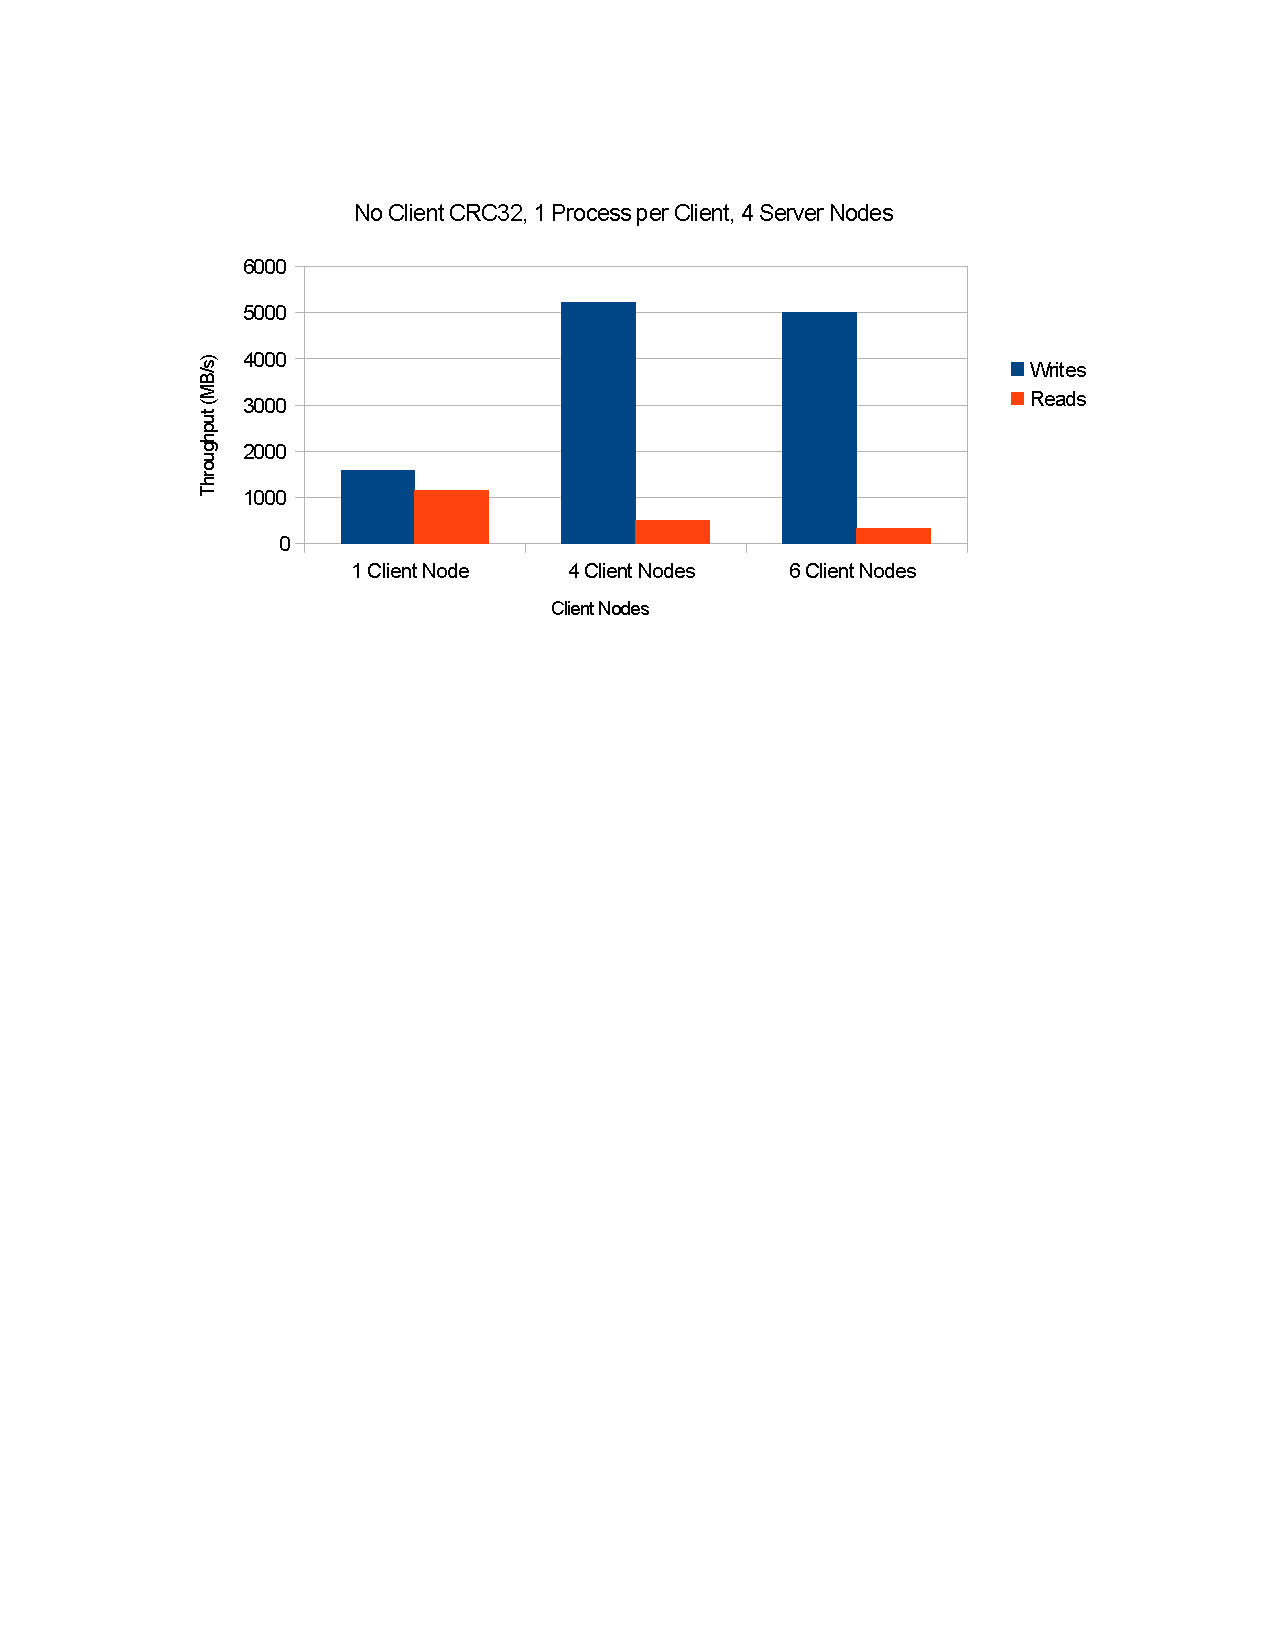
\includegraphics[width=3.5in]{ior-client-no-crc32}
%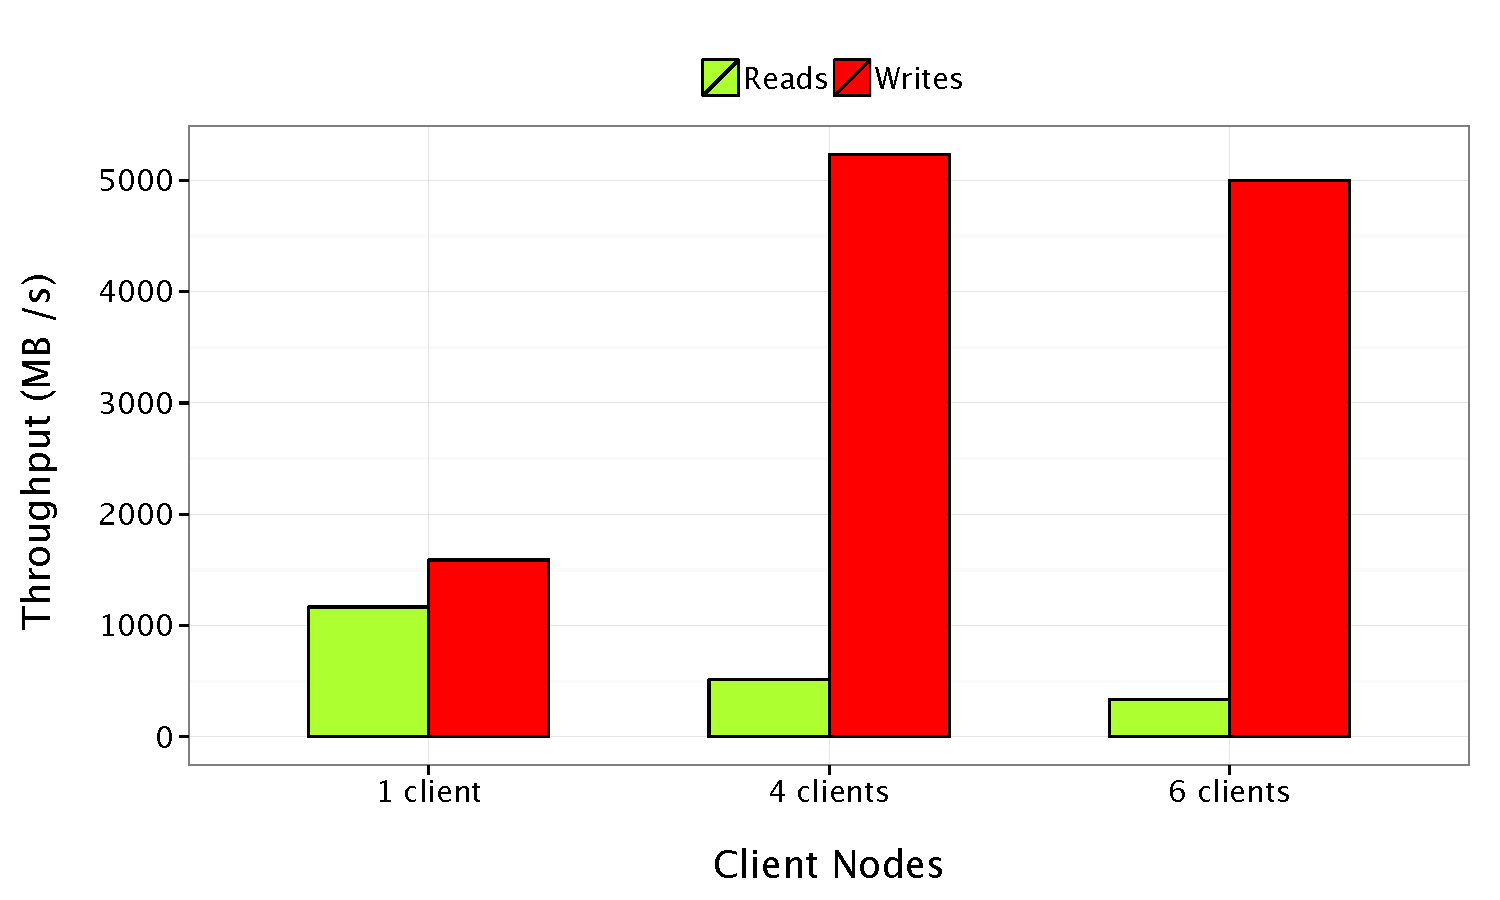
\includegraphics[width=3.5in]{ior_no_crc}
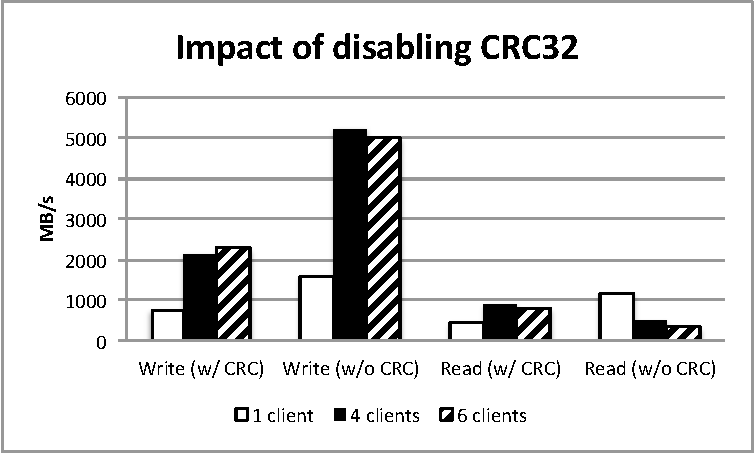
\includegraphics[width=3.5in]{crc32}
\caption{Impact of Disabling CRC32}
\label{fig:ior-no-client-crc32}
\end{figure}

We observed that IOR write throughput increased dramatically and is now very
close and comparable to the RADOS Bench performance. Read performance continued
to be poor and continued to scale inversely with the increasing number of
client processes.  Please note that, since these tests were performed, Inktank
has implemented SSE4-based CRC32 code for Intel CPUs.  While any kernel based
CRC32 processing should have already been using SSE4 instructions on Intel
CPUs, this update will allow any user-land Ceph processes to process CRC32
checksums with significantly less overhead.

\subsubsection{Improving IOR Read Performance}

Deeper analysis with \verb!perf! showed that there was heavy lock contention
during parallel compaction in the Linux kernel memory manager.  This behavior
was first observed roughly in the kernel 3.5 time frame which was the kernel
installed on our test systems.\footnote{For more information,
please refer to \url{http://lwn.net/Articles/517082/} and
\url{https://patchwork.kernel.org/patch/1338691/}.}  We upgraded our test
systems with kernel version 3.9 and performed RADOS Bench test.  The results
%were dramatic:  read performance improved from 4678 MB/s to 8643 MB/s (almost
were dramatic:  read performance improved from 4678 MB/s to 7499 MB/s 
(a 60\% improvement).  Write performance was also fractionally improved from
4720 MB/s to 5284 MB/s (a 12\% improvement).
%extremely positive and presented in
%Figure~\ref{fig:rados-kernel}. As can be seen, with the 3.9 kernel, while
%there was a slight improvement on write performance, read performance improved
%dramatically.  In addition to the kernel change, the amount of CephFS client
%kernel read-ahead cache size was increased as well.


%\begin{figure}[htb]
%\centering
%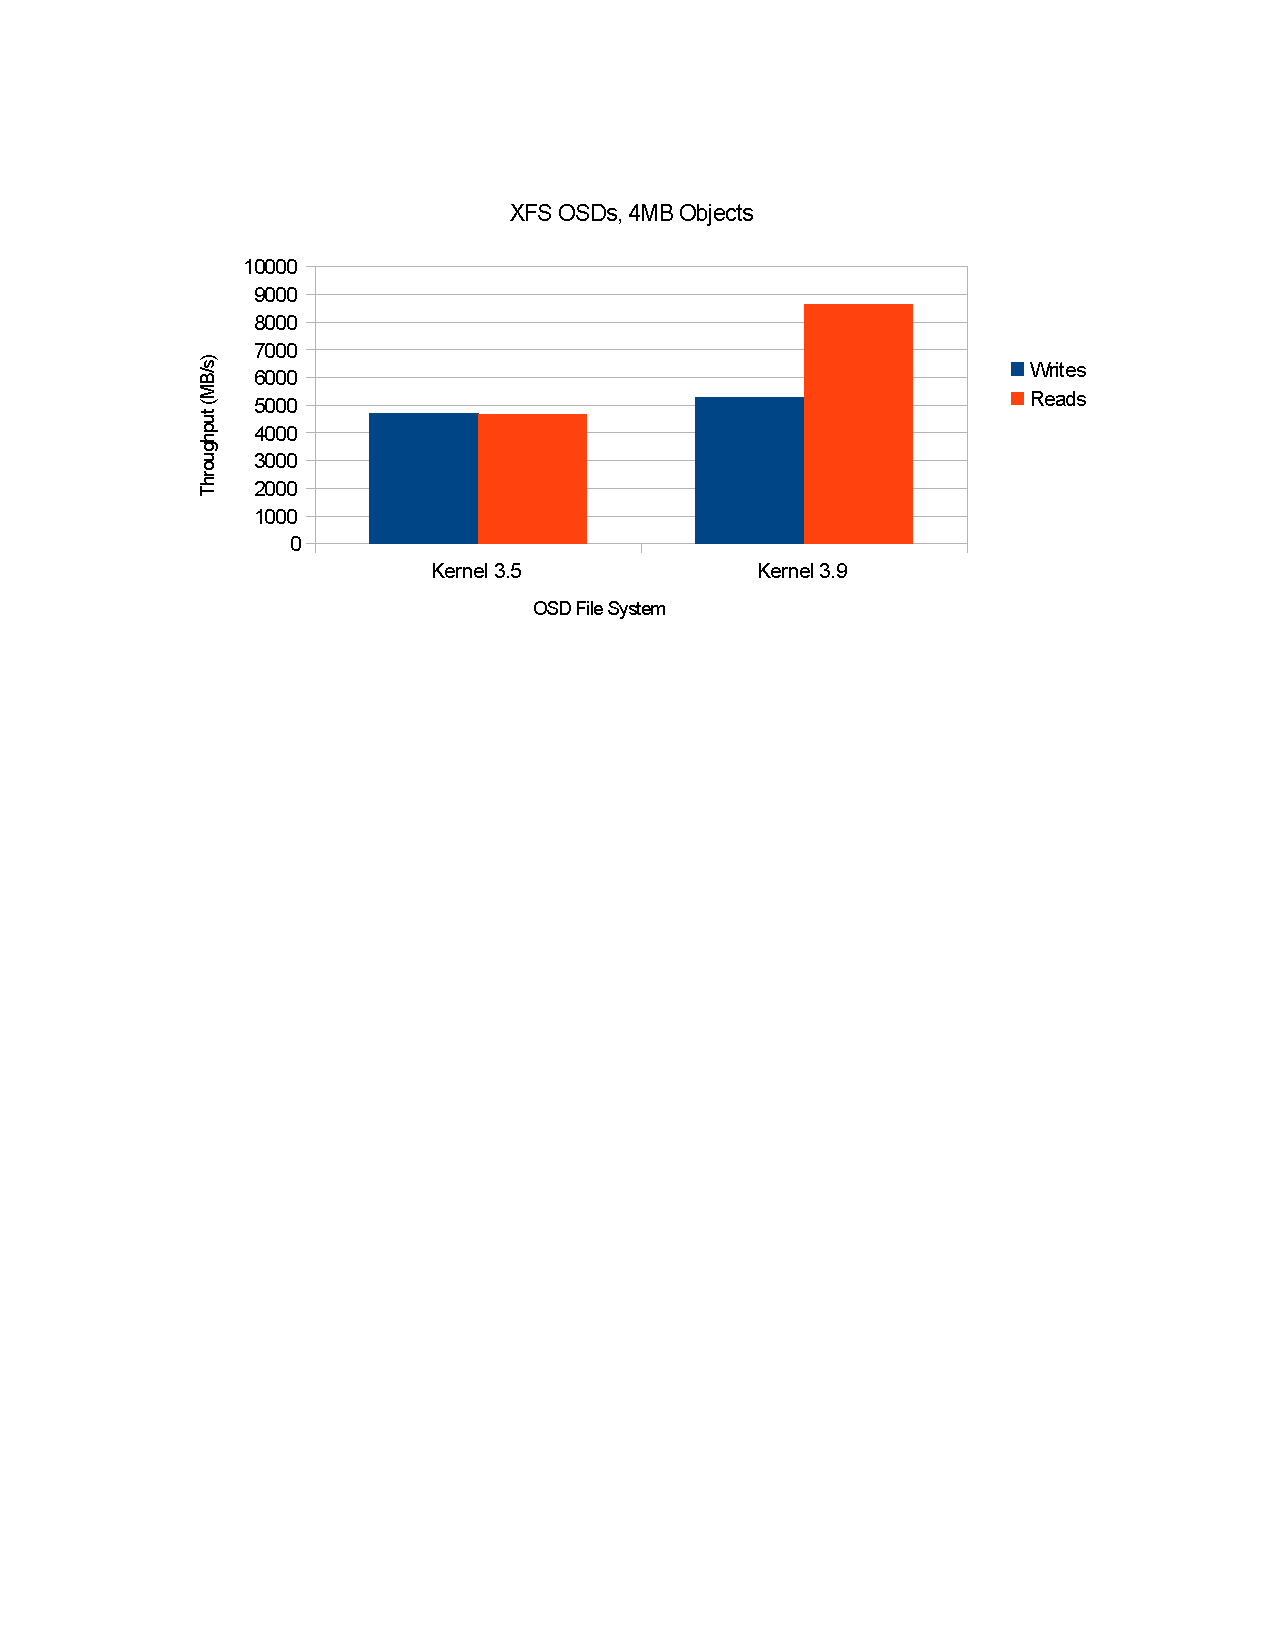
\includegraphics[width=3.5in]{rados-kernel-35vs39}
%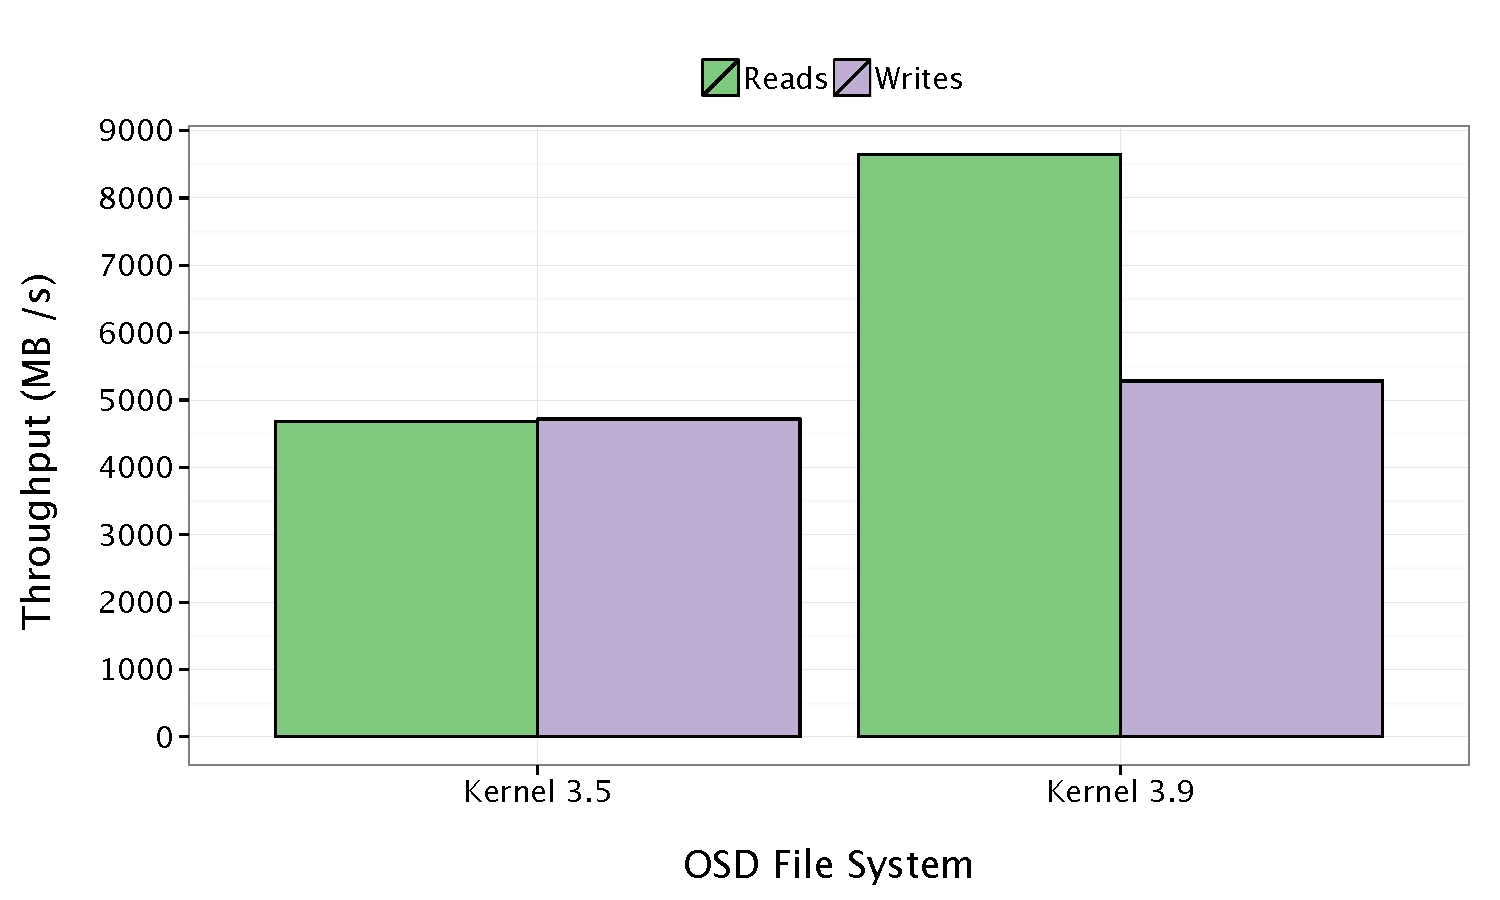
\includegraphics[width=3.5in]{rados_kernel}
%\caption{RADOS bench: Linux kernel version 3.5 vs. 3.9}
%\label{fig:rados-kernel}
%\end{figure}



%%%%%%%%%%%%%%%%%%%%%%%%%%%% REMOVED to save space

%\begin{Verbatim}[samepage=true, fontsize=\small]
%mount -t ceph 10.37.248.43:6789:/ 
%  /mnt/ceph -o name=admin,nocrc,
%  readdir_max_bytes=4104304,
%  readdir_max_entries=8192
% \end{Verbatim}

%% SCOTT - is figure 15 IOR over Ceph and 14 is RADOS bench? If so, can we
%% mention that 15 shows the filesystem performance?

Additionally, we increased the size of the CephFS kernel client's read-ahead
cache.  
%IOR results reflecting the read-ahead cache size change are presented in
%Figure~\ref{fig:ior-kernel-39}.

\begin{comment}
\begin{figure}[htb]
\centering
%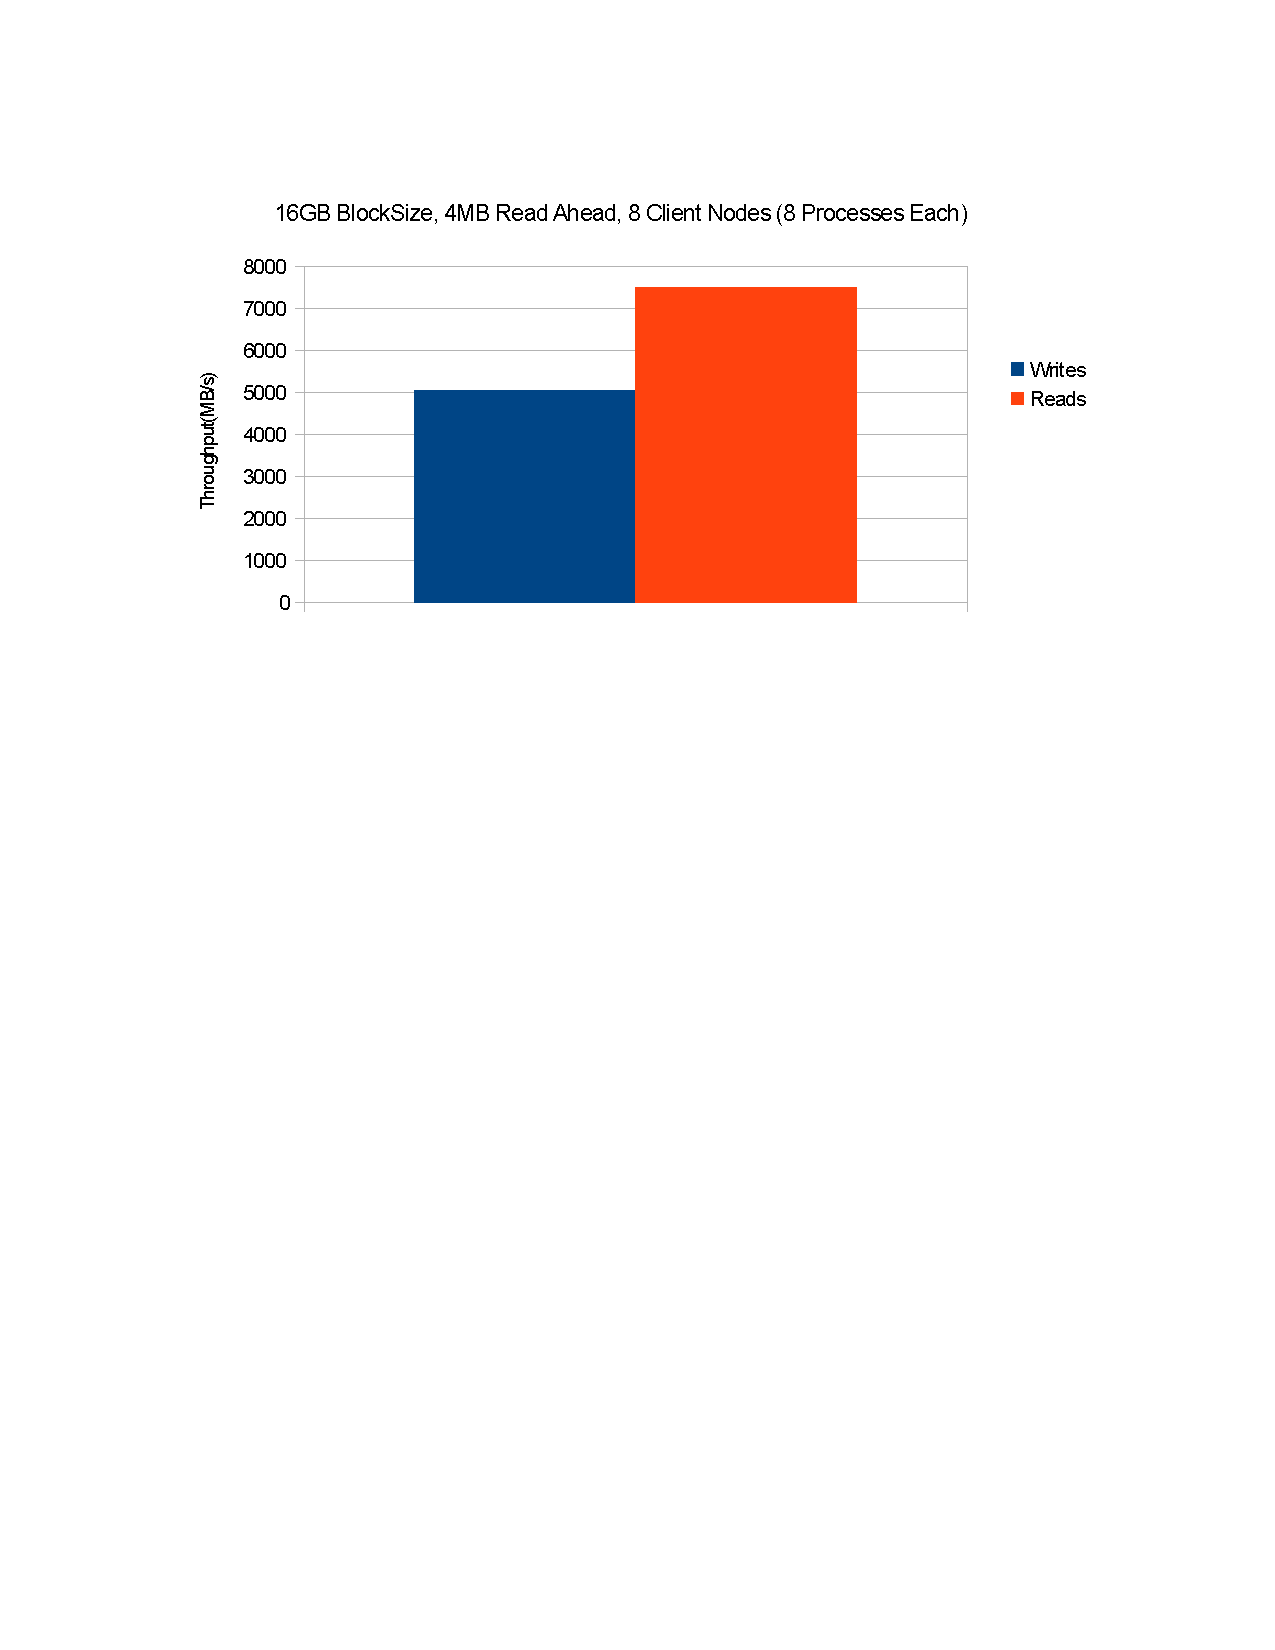
\includegraphics[width=3.5in]{ior-kernel-39}
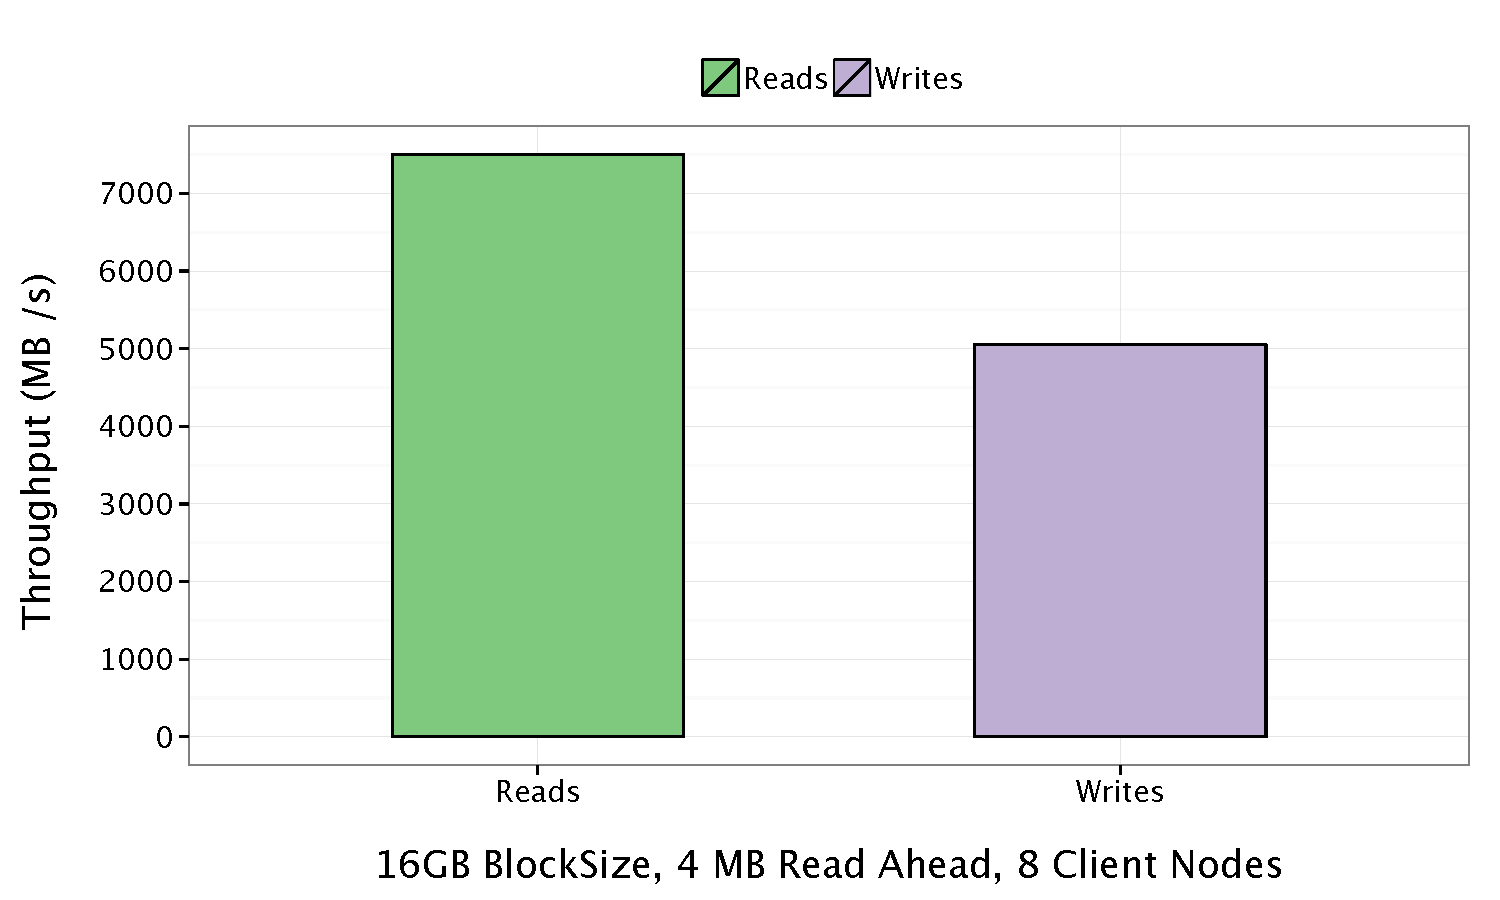
\includegraphics[width=3.5in]{ior_kernel_change}
\caption{CephFS performance with kernel changes to 3.9, IOR with 4 MB transfer
size}
\label{fig:ior-kernel-39}
\end{figure}
\end{comment}

By installing a newer kernel, increasing read-ahead cache size, and increasing
the number of client IOR processes, we were able to achieve very satisfactory
I/O performance at the Ceph file system-level.


\subsubsection{Repeating the IOR Scaling Test}

As before, we ran IOR scaling tests with two cases: transfer size 4 KB and 4
MB.  These results are illustrated in Figure~\ref{fig:ior-064}, respectively.
As expected, we saw both improved read and write performance. These new read
and write performance are in line with observed RADOS bench performance.

%% SCOTT - Can we use the same Y axis for these figures? Any comment from Inktank
%% as to why 4 KB performance is better than 4 MB performance?

\begin{figure}[htb]
\centering
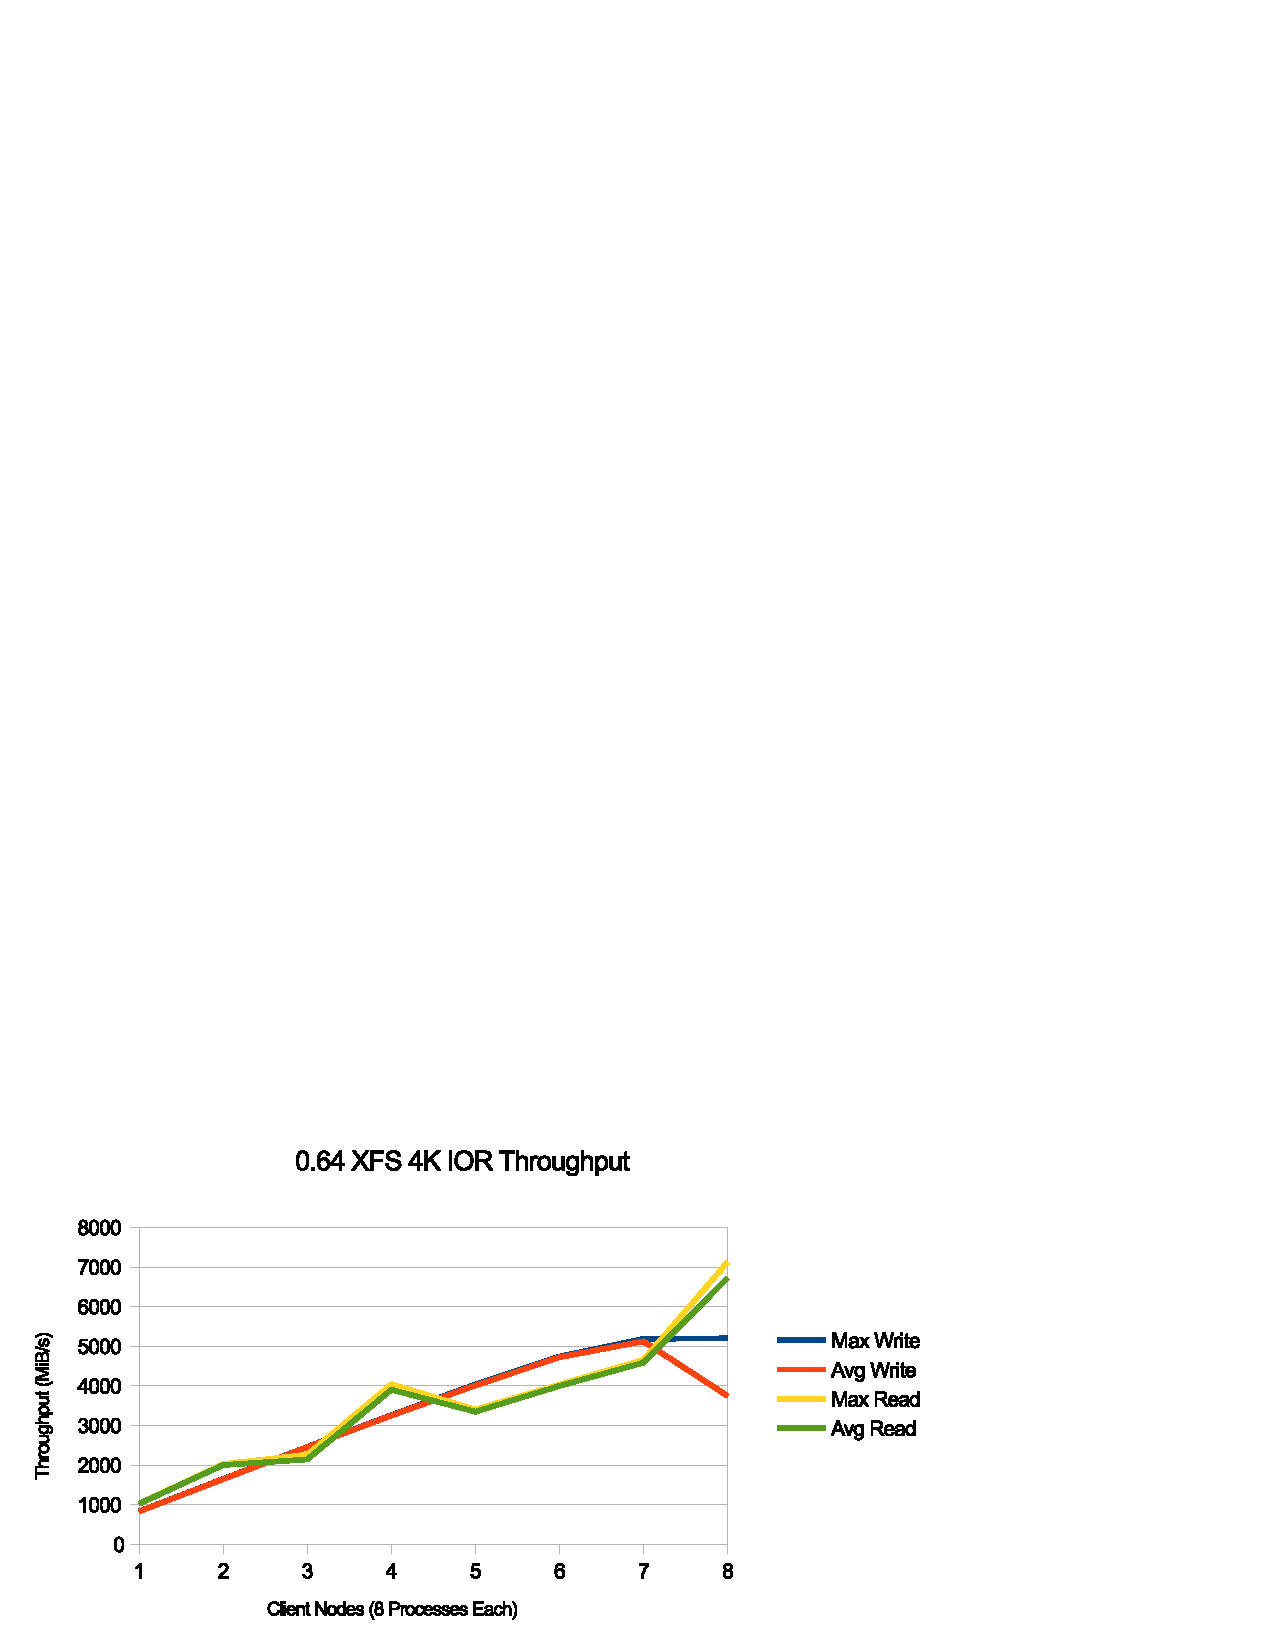
\includegraphics[width=3.5in]{ior-064-4k}
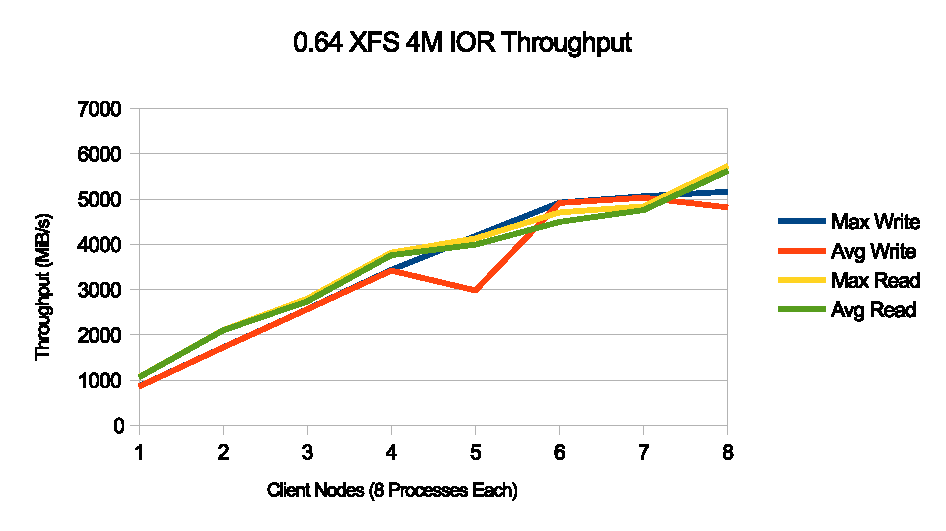
\includegraphics[width=3.5in]{ior-064-4m}
\caption{IOR Scaling Test: 4 KB and 4 MB transfer size}
\label{fig:ior-064}
\end{figure}

%Throughout our IOR testing, we observed that the average write throughput is
%lower than the maximum.  
% This behavior was observed during other tests as well,
%indicating that we may have periods of time where write throughput is
%temporarily degrading.  Despite these issues, performance generally seems to be
%improving with respect to increasing number of clients.  

Writes seem to be topping out at around 5.2 GB/s (which is roughly what we
would expect due to journaling effectively halving the write performance).
Reads seem to be topping out anywhere from 5.6-7 GB/s, however it is unclear
if read performance would continue scaling with more clients and get closer to
8 GB/s we observed with RADOS Bench.

\begin{comment}
\subsection{Metadata Performance Tuning}
For brevity's sake, we are omitting most of our file and directory creation
rate results.  However, over the course of our testing we did notice that in
CephFS 0.64 a significant improvement in the performance of file creation with
mdtest.  Shown in Figure~\ref{fig:mdtest-064-file-create}, we note
that as number of clients increase, the file creation rate does not scale
linearly, which suggested some form of lock contention.  Due to the large
differences in the initially observed performance, and the performance with
Ceph 0.64, opportunities for file and directory create tuning may be
substantial. 

\begin{figure}[htb]
\centering
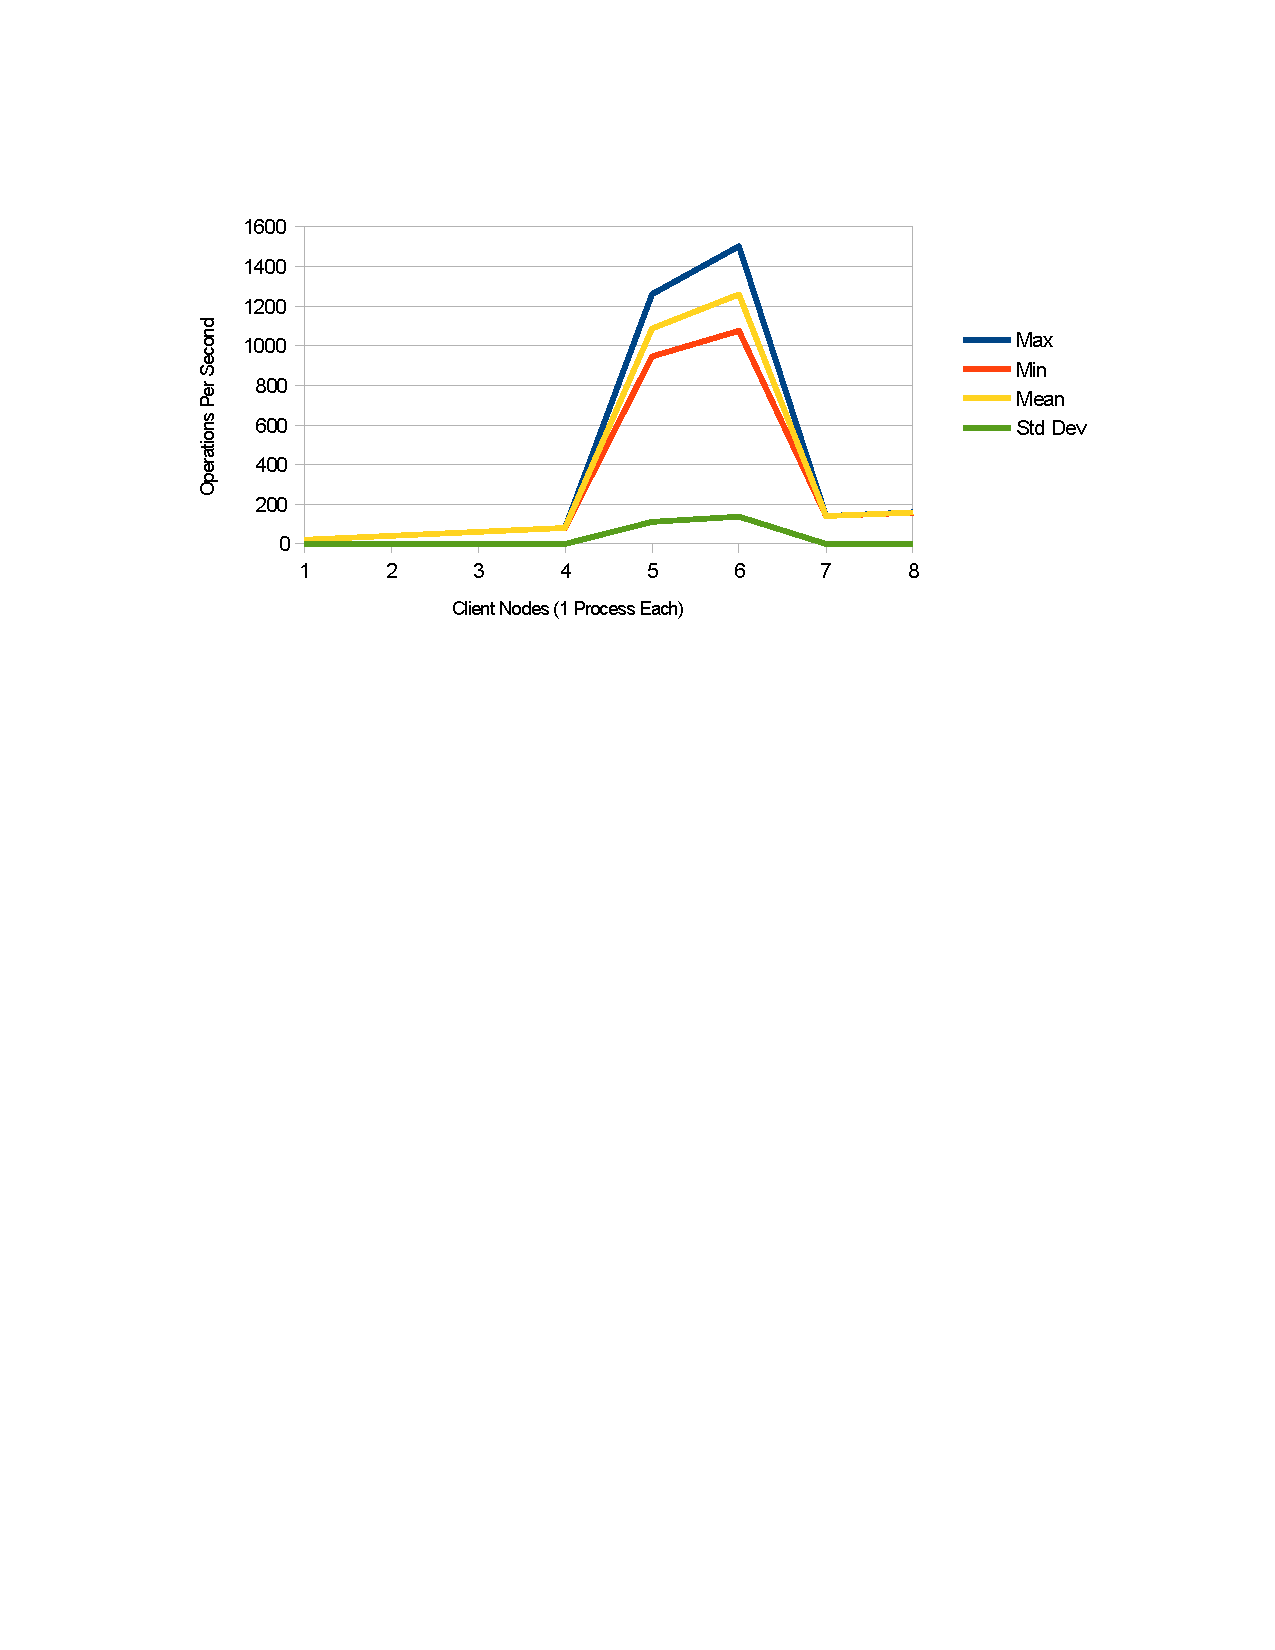
\includegraphics[width=3.5in]{mdtest-064-file-create}
\caption{mdtest of file creation on Ceph 0.64}
\label{fig:mdtest-064-file-create}
\end{figure}

\end{comment}
